%----------------------------------------------------------------------------------------
%	PACKAGES AND OTHER DOCUMENT CONFIGURATIONS
%----------------------------------------------------------------------------------------

\documentclass[11pt]{article}
\usepackage{graphicx}
\usepackage[utf8]{inputenc}  
\usepackage[T1]{fontenc} 
\usepackage[top=2cm,bottom=2cm,left=1.3cm,right=1.5cm,asymmetric]{geometry}
\usepackage{amsfonts}
\usepackage{graphicx}
\usepackage{caption}
\usepackage{subcaption}
\usepackage{float}
\usepackage{subfig}
\usepackage{algorithm}
\usepackage{algpseudocode}
\usepackage{fancyhdr}
\usepackage{ stmaryrd }
\usepackage{placeins}
\usepackage{ amssymb }
\usepackage{mathtools}
\pagestyle{fancy}
\renewcommand{\footrulewidth}{1pt}
\fancyhead[R]{\textit{Master MVA : Reinforcement Learning}}
\fancyfoot[L]{\textit{}}
%\usepackage{unicode-math}
%\setmathfont{XITS Math}
%\setmathfont[version=setB,StylisticSet=1]{XITS Math}
\usepackage{array,multirow,makecell}
\setcellgapes{1pt}
\makegapedcells
\newcolumntype{R}[1]{>{\raggedleft\arraybackslash }b{#1}}
\newcolumntype{L}[1]{>{\raggedright\arraybackslash }b{#1}}
\newcolumntype{C}[1]{>{\centering\arraybackslash }b{#1}}

\pagestyle{fancy}
\renewcommand{\footrulewidth}{1pt}
\fancyfoot[L]{\textit{}}

\newcommand{\argmin}{\operatorname{arg min}}

\newtheorem{definition}{Definition}
\newtheorem{theorem}{Theorem}
\newtheorem{lemma}{Lemma}
\newtheorem{corollary}{Corollary}
\newtheorem{proposition}{Proposition}

\setlength{\parindent}{0pt}
   

\begin{document}

\parskip 6pt

\begin{center}
\section*{Final project - Reinforcement Learning}
\section*{Stochastic versus adversarial bandits}
\large{Isabella Joanna Lukasewitz \& Sammy Khalife}
\end{center}

\section*{Introduction}
Multi-armed bandit games are a simple model for sequential decision making that has been studied extensively from the second half of the last century on and that remains to be an important subject of research. The basic framework presents a player in a situation of sequential decision making. After each decision (out of a discrete and finite decision set) he receives a feedback from the environment in the form of a reward (or loss). The crucial tradeoff faced is the one between \textit{exploration} and \textit{exploitation}: While exploring the possible decision arms in order not to take suboptimal decisions, he/she should exploit what is already known in the best possible way. The performance of a strategy is usually measured as the regret with respect to a certain benchmark where the benchmark is generally given by the best fixed strategy throughout the game (to be defined more precisely in different scenarios).

For a long time, two main frameworks have been considered in the literature, largely independently from each other. The stochastic case assumes fixed underlying distributions for the respective decision arms (\cite{Thom33}, \cite{Robb85}, \cite{Auer02a}). The more general and therefore more difficult adversarial case (\cite{Auer95},  \cite{Auer02b}) does not make such an assumption. Rewards are assumed to be generated entirely randomly and fully determined given a sequence of decisions ahead of the game (while being obviously unknown to the player).

For both scenarios, algorithms have been developed with optimal worst-case guarantees. In a stochastic environment, the UCB1 algorithm (\cite{Auer02a}) for instance attends a regret of $O(\log n)$ while in the adversarial case $O(\sqrt{n})$ is reached by EXP3 (\cite{Auer02b}) for bounded rewards. However, generally algorithms designed for the stochastic framework fail completely in the adversarial one while algorithms adapted to the adversarial framework do not manage to take advantage of the "nice" stochastic case. Moreover, no frameworks different from the "extreme" adversarial and stochastic one have been considered.

Attempts to combine the two have been made only recently. In this article we aim first to provide a short overview of the most popular algorithms considered until today, their performance and their regret guarantees. In the second part, we will analyze more closely two algorithms proposed for the two frameworks jointly, the SAO algorithm (Bubeck et al., 2012 \cite{Bube12}) and the so-called EXP3++ (Seldin et al, 2014 \cite{Seld14}). Finally, we will present an algorithm that was proposed recently by Sani et al. \cite{Sani14}. It has been developed for a more general decision problem with full feedback. We will adapt it to the bandit framework and test its performance therein.

\section*{Multi-armed bandit environments}
Let $r_{t}^{A_{t}}$ be the reward obtained at time $t$ by pulling arm $A_{t}$. We will consider four different environments, following in that Seldin et al. \cite{Seld14}. In all cases, rewards are assumed to be bounded in $[0,1]$. The expected regret to be minimized is a priori defined as the difference between the expected loss of the algorithm up to round $t$ and the expected loss of the best arm up to round $t$:
$$\mathbb{E}[R(t)]=\max_{a}\{ \sum_{s=1}^{t} \mathbb{E}[r_{s}^{a}]\}-\sum_{s=1}^{t} \mathbb{E}[r_{s}^{A_{s}}].$$
The expectation is taken over the possible randomness of the algorithm and loss generation model. 

In the \textbf{adversarial regime}, the rewards are generated by an ''unrestricted adversary'' (oblivious to the algorithm's actions). This is the most general case. The regret is a posteriori computed as the difference to the best fixed strategy in hindsight: 
$$ R(t)=\max_{a}\{ \sum_{s=1}^{t} r_{s}^{a} \}-\sum_{s=1}^{t} r_{s}^{A_{s}}.$$

In the \textbf{stochastic regime}, we suppose that the rewards are sampled independently with respect to a distribution that does not depend on time, then $\mathbb{E}[r_{s}^{a}]=\mu_{a}$, and the regret simplifies : 
$$\mathbb{E}[R(t)]=t\max_{a}\mu_{a}-\sum_{s=1}^{t} \mathbb{E}[r_{s}^{A_{s}}]$$
which can be written as
$$\mathbb{E}[R(t)]=\sum_{a}\mathbb{E}[N_{t}(a)]\Delta_{a}$$ 
where $\Delta(a)=(\max_{a'}\mu_{a'})-\mu_{a}$ and $N_{t}(a)$ is the number of time a has been pulled until time t.

Seldin et al. introduce two new frameworks that can be regarded as in between the aforementioned ones.

The first of them is called \textbf{adversarial regime with a gap}, which is an adversarial regime for which we suppose that there exists a round $\tau$ and an arm $a_{\tau}*$ such that for any $t \geq \tau$, $a_{\tau}*$ persists to be the best arm in hindsight for all rounds $t \geq \tau$, i.e $\forall \, t \geq \tau$,  $a_{\tau}* \in \argmin_{a'}(\sum_{s=1}^{t}l_{s}^{a'})$.

The \textbf{contamined stochastic regime} is a stochastic regime with adversarial elements. The adversary chooses some pairs $(t,a)$ (''locations'') before the game starts and assigns their rewards in an arbitrary way. The rest of the rewards are generated as in the stochastic framework.

\section*{Popular bandit algorithms - an overview}

In this section we will give a short overview of the algorithms treated in class and compare their performance on several bandit problems. Since a lot of this material has been already treated throughout the course, we will keep the presentation short. Please note that all of the algorithms can be found in Appendix A. 

\subsection*{Stochastic framework}

The stochastic framework was the first one to be treated in multi-armed bandit problems. The Thompson algorithm, a very efficient algorithm for problems following the stochastic assumption, was already proposed in 1933 but was to be rediscovered many decades later \cite{Thom33}. A very popular basic learning algorithm is the UCB algorithm proposed by Auer et al. in \cite{Auer02a}.

It has been shown that the UCB achieves an essentially optimal regret of $O(\log n)$ (it matches the Lai-Robbins lower bound up to logarithmic factors). We recall this fact in the following theorem.
\begin{theorem}
The expected regret of the UCB algorithm is bounded as
$$ \mathbb{E}[R(t)] = \sum_{a}\mathbb{E}[N_{t}(a)]\Delta_{a} <
 6 \sum_{a: \, \Delta_a > 0} \frac{\log t}{\Delta_a} + K (\frac{\pi^2}{3} + 1).$$
\end{theorem}



\subsection*{Adversarial framework}




\section*{"The best of both worlds": The SAO algorithm}

There has only been very recently attempts to overcome the distinction between the two aforementioned frameworks. The first one was made by Bubeck et al. in 2012 \cite{Bube12}, where they introduced the so-called SAO algorithm. This algorithm manages in a certain way to bridge the gap between the two worlds: It has a build-in mechanism to detect the framework the player is in. However, it does not explicitly leave room for scenarios that are not purely stochastic or purely non-stochastic. This further extension will be tackled by the EXP3++ algorithm in the following section.

The SAO algorithm starts off like a classical algorithm for the stochastic framework, interleaving an \textit{exploration} and an \textit{exploitation} phase. At the beginning, all arms are activated and are sampled with the same probability. In the course of the algorithm, more and more arms get gradually deactivated (their sampling probability decreases smoothly) and the remaining arms are sampled with steadily increasing probability. The algorithm thus moves gradually from an exploration to a exploitation strategy. At each point in time, certain consistency conditions are checked to ensure that the assumed stochastic framework holds. As soon as one of these conditions fails, the algorithm assumes an adversarial framework and switches to the EXP3.P algorithm. This algorithm, based directly on the EXP3 algorithm, was equally proposed in \cite{Auer02b}. It introduces a biased estimate of the cumulative gain and exhibits advantageous theoretical properties when deriving high-probability bounds.

An an important novelty, they mange to prove an $\tilde{O}(\sqrt{n})$ regret bound for the adversarial case and a $polylog(n)$ bound for the stochastic case, thus coming close to the theoretical performance bounds for the UCB and the EXP3 algorithm that we recalled in the previous section. Their main result reads as follows:
\begin{theorem}
There exists an algorithm SAO for the MAB problem such that:
\begin{enumerate}
\item[(a)] in the adversarial model, SAO achieves regret $\mathbb{E}[R_n] \leq O(\sqrt{nK} \log^{3/2}(n) \log K)$.
?\item[(b)] in the stochastic model, SAO achieves regret $\mathbb{E}[R_n] \leq O(K \log^{2}(n) \log K)$.\end{enumerate}
\end{theorem}

The details are stated in the following theorem. The algorithm (with the explanation of the parameters) can be found in the appendix.
\begin{theorem}
SAO with $\beta = n^4$ satisfies in the stochastic model:
$$ \mathbb{E}[R_n] \leq O \left (\frac{K \log(K) \log^2(n)}{\Delta} \right),$$
and in the adversarial model:
$$\mathbb{E}[R_n] \leq O(\log(K) \log^{3/2}(n) \sqrt{nK}).$$
More precisely, for any $\delta \in (0,1)$, with probability at least $1-\delta$, SAO with $\beta = 10Kn^3 \delta^{-1}$ satisfies in the stochastic model:
$$\bar{R}_n = \frac{260K (1 + \log K) \log^2(\beta)}{\Delta},$$
and in the adversarial model:
$$R_n = \leq 60(1 + \log K) (1 + \log n) \sqrt{nK \log(\beta) + 5 K^2 \log^2(\beta)} + 200K^2 \log^2(\beta).$$
\end{theorem}

\subsection*{Numerical experiments}

We have tested the performance of the algorithm in comparison to several standard algorithms that were brought up in the last section. To our knowledge, this has not been done before, mainly because Bubeck et al. state themselves that a practical implementation of the algorithm should encompass some enhancements like an extension to a mixed stochastic-adversarial environment. As expected, the performance does therefore not quite match the one of the benchmarks. In several examples, we can see however how the algorithm actually manages to bridge the gap better than the current standard.


\section*{An adapted EXP3 algorithm}

As a reminder, the EXP3 algorithm is made as follows : 
\FloatBarrier
\begin{algorithm}
\caption{EXP3}\label{RS}
Given fixed exploitation parameter $\eta$ and exploration parameter $\beta$\\
$\forall$ a $\omega_{a}(1)=1$\\
1. for t=2:$T_{end}$\\
2. $p_{a}(t) = (1-\beta)\frac{\omega_{a}(t-1)}{\sum_{a}\omega_{a}(t-1)}+\frac{\beta}{K}$\\
3. $A_{t}$ drawn with $p_{a}(t)$ distribution on arms\\
4. $\tilde{r}_{A_{t}} = \frac{r_{A_{t}}}{p_{A_{t}}(t-1)}$ and update of $\omega$ on $A_{t}$ only : $\omega_{A_{t}}(t)=\omega_{A_{t}}(t-1)exp(\eta \tilde{r}_{A_{t}(t)})$\\
\end{algorithm}
\FloatBarrier
~\\
The EXP3 algorithm (Auer et al., 2002) is very efficient for adversarial frameworks, but has some difficulties to adapt to every kind of problems. Below the regrets in a stochastic framework compared with one of the most efficient algorithm in this case (Thompson sampling) :
\begin{center} \textbf{Comparaison of Thompson and EXP3 on stochastic framework}\end{center}
 \begin{figure}[!h]
   \begin{minipage}[c]{0.5 \linewidth}
   \centering
    \captionsetup{justification=centering,margin=1cm}
      \includegraphics[width=9cm]{Thompson_vs_exp3.jpg}
      \caption{''Easy problem''\\KL complexity = 6.3 (6 arms) $\beta=0.01$, $\eta$=0.01}
   \end{minipage} \hfill
   \begin{minipage}[c]{0.5 \linewidth}
   \centering
   \captionsetup{justification=centering,margin=1cm}
      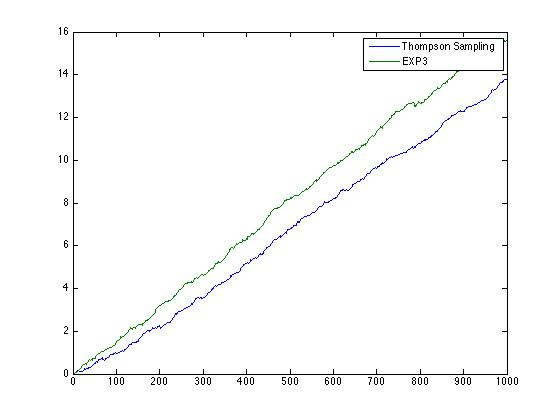
\includegraphics[width=9cm]{complexPbVs.jpg}
      \caption{''Difficult problem'',\\KL complexity = 315 (10 arms) $\beta$=0.01, $\eta$=0.01}
   \end{minipage} 
\end{figure}
~\\
To adapt EXP3 to stochastic configurations, the idea of the algorithm named EXP3++ (cf [1]) is to replace the exploration parameter $\beta$ and exploitation parameter $\eta$ by new time-depending parameters.
~\\
\FloatBarrier
\begin{algorithm}
\caption{EXP3++}\label{RS}
$\forall$ a $\tilde{L}_{0}(a)=0$\\
1. for $t=1:T_{end}$~\\
2. $\forall$ a $\in \{1,..K\}$\\
 $\epsilon_{t}(a)=min\{\frac{1}{2K}, \beta_{t}, \xi_{t}(a)\}$ \\
$\rho_{t}(a)=exp(-\eta_{t}\tilde{L}_{t-1}(a))/\sum_{a'}exp(-\eta_{t}\tilde{L}_{t-1}(a'))$\\
$\tilde{\rho}_{t}(a)=(1-\sum_{a'}\epsilon_{t}(a'))\rho_{t}(a)+\epsilon_{t}(a)$\\
3. Draw action $A_{t}$ with the $\tilde{\rho}_{t}$ distribution on arms.~\\
4. Observe the loss $l_{t}^{A_{t}}$ and $\forall$ a $\in \{1,..,K\}$\\
$\tilde{l}_{t}^{a}=\frac{l_{t}^{A_{t}}}{\tilde{\rho}_{t}(a)} \textbf{1}_{A_{t}=a}$\\
$\tilde{L}_{t}(a)=\tilde{L}_{t-1}(a)+\tilde{l}_{t}^{a}$
\end{algorithm}
\FloatBarrier~\\
With $\eta_{t}=2\beta_{t}$ and $\xi_{t}(a)=0$ we find back EXP3.


\section*{Theoretical results for EXP3++}
The main results have been demonstrated by Seldin et al. \cite{Seld12}.

\subsection*{Adversarial regimes}

\begin{theorem}
For $\eta_{t}=\beta_{t}$ and $\xi(t) \geq 0$, the regret for any $t\geq0$ satisfies $$R(t) \leq 4\sqrt{K\ln K}$$ This upper bound is two times above the EXP3 theoretical upper bound.
\end{theorem}

\subsection*{Stochastic regime}
First, if one supposes that we know the gaps, EXP3++ allows by defining adapted $\xi_{t}$ and $\eta_{t}$ to control the regret. In practice the gaps are not known and one will use an emprirical estimator : $$\hat{\Delta}_{t}(a)=min\{1,\frac{1}{t}(\max_{a'}(\tilde{L}_{t}(a')-\tilde{L}_{t}(a))\}$$
\begin{theorem}
Knowing the gaps $\Delta(a)$, with $\xi_{t}(a)=\frac{c\ln(t\Delta(a)^{2})}{t\Delta(a)^{2}}$, the regret satisfies :
$$R(t) \leq \sum_{a} O(\frac{\ln(t)^{2}}{\Delta(a)})+\sum_{a}\tilde{O}(\frac{K}{\Delta(a)^{3}})$$
\end{theorem}

\begin{theorem}
Let us consider the empirical gap $\Delta_{t}(a)$ defined previously, a time $t^{*}$ such that $t^{*}\geq \frac{4c^{2}K\ln(t*)^{4}}{\ln(K)}$ and let $t^{*}(a)=max\{t*,\lceil e^{1/\Delta(a)^{2}}\rceil\}$.
Then by tuning $\xi_{t}(a)=\frac{c\ln(t)^{2}}{t\hat{\Delta}_{t-1}(a)^{2}}$ (giving the EXP3$++^{AVG}$ algorithm) the regret in the stochastic regime satisfies :
$$R(t) \leq \sum_{a}O(\frac{\ln(t)^{3}}{\Delta{a}})+\sum_{a}\Delta(a)t^{*}(a)$$
\end{theorem}

\subsection*{Contamined stochastic regime}

\begin{theorem}
With the same assumptions as theorem 3 except $t^{*}(a)=max\{t^{*}, \lceil e^{4/\Delta(a)^{2}}\rceil \}$, the regret satisfies :
$$R(t) \leq \sum_{a}O(\frac{\ln(t)^{3}}{\Delta(a)})+\sum_{a}max\{t^{*}(a),\tau\}$$
\subsection*{Adversarial regime with a gap}
\textbf{Theorem 5} With the same assumptions as in theorem 3, the regret satisfies :
$$R(t) \leq \sum_{a}\{\min_{\tau}\{max\{t^{*},\tau,e^{1/(\Delta(\tau,a))^{2}}\}+O(\frac{\ln(t)^{3}}{\Delta(\tau,a)})\}$$~\\
\end{theorem}

With $\eta_{t}=\beta_{t}$, the EXP3++ algorithm provides a guarantee against adversarial situations. On the other hand, a configuration such that $\eta=1$ provide better results on a stochastic configuration. Still a lot has to be done concerning this trade-off.

\section*{Numerical comparison}


\section*{The $(\mathcal{A},\, \mathcal{B})-$PROD algorithm applied to multi-armed bandits}

The multi-armed bandit problem is a special case of a general online decision-making problem. It belongs to the class of partial feedback problems: In an MAB, the player's feedback is equal to his reward. He does in particular not obtain any knowledge regarding the theoretical rewards of the arms he has not played.

\pagebreak

\begin{thebibliography}{1}

\bibitem{Auer95} P. Auer, N. Cesa-Bianchi, Y. Freund and R.E. Schapire (1995). {\em Gambling in a rigged casino: The adversarial multi-armed bandit problem}. In Proceedings of the Annual Symposium on Foundations of Computer Science.

\bibitem{Auer02a} P. Auer, N. Cesa-Bianchi and P. Fischer (2002). {\em Finite-time analysis of the multiarmed bandit problem}. Machine Learning, 47.

\bibitem{Auer02b} P. Auer, N. Cesa-Bianchi, Y. Freund and R.E. Schapire (2002). {\em The nonstochastic multiarmed bandit problem}. SIAM Journal of Computing, 32(1).

\bibitem{Bube12} S. Bubeck and A. Slivkins (2012). {\em The best of both worlds: stochastic and adversarial bandits}. In Proceedings of the International Conference on Computational Learning Theory (COLT).

\bibitem{Lai85} T.L. Lai and H. Robbins (1985). {\em Asymptotically efficient adaptive allocation rules}. Advances in Applied Mathematics, 6.

\bibitem{Robb52} H. Robbins (1952). {\em Some aspects of the sequential design of experiments}.  Bulletin of the American Mathematical Society.

\bibitem{Sani14} A. Sani, G. Neu and A. Lazaric (2014). {\em Exploiting easy data in online optimization}.  Advances in Neural Information Processing Systems.

\bibitem{Seld14} Y. Seldin and A. Slivkins (2014). {\em One practical algorithm for both stochastic and adversarial bandits}.  Proceedings of the 31st International Conference on Machine Learning (ICML-14).

\bibitem{Thom33} W.R. Thompson (1933). {\em On the likelihood that one unknown probability exceeds another in view of the evidence of two samples}. Biometrika, 25.

\end{thebibliography}

\end{document}